
%% LyX 2.2.1 created this file.  For more info, see http://www.lyx.org/.
%% Do not edit unless you really know what you are doing.
\documentclass[12pt]{beamer}\usepackage[]{graphicx}\usepackage[]{color}
%% maxwidth is the original width if it is less than linewidth
%% otherwise use linewidth (to make sure the graphics do not exceed the margin)
\makeatletter
\def\maxwidth{ %
  \ifdim\Gin@nat@width>\linewidth
    \linewidth
  \else
    \Gin@nat@width
  \fi
}
\makeatother

\definecolor{fgcolor}{rgb}{0.345, 0.345, 0.345}
\newcommand{\hlnum}[1]{\textcolor[rgb]{0.686,0.059,0.569}{#1}}%
\newcommand{\hlstr}[1]{\textcolor[rgb]{0.192,0.494,0.8}{#1}}%
\newcommand{\hlcom}[1]{\textcolor[rgb]{0.678,0.584,0.686}{\textit{#1}}}%
\newcommand{\hlopt}[1]{\textcolor[rgb]{0,0,0}{#1}}%
\newcommand{\hlstd}[1]{\textcolor[rgb]{0.345,0.345,0.345}{#1}}%
\newcommand{\hlkwa}[1]{\textcolor[rgb]{0.161,0.373,0.58}{\textbf{#1}}}%
\newcommand{\hlkwb}[1]{\textcolor[rgb]{0.69,0.353,0.396}{#1}}%
\newcommand{\hlkwc}[1]{\textcolor[rgb]{0.333,0.667,0.333}{#1}}%
\newcommand{\hlkwd}[1]{\textcolor[rgb]{0.737,0.353,0.396}{\textbf{#1}}}%
\let\hlipl\hlkwb

\usepackage{framed}
\makeatletter
\newenvironment{kframe}{%
 \def\at@end@of@kframe{}%
 \ifinner\ifhmode%
  \def\at@end@of@kframe{\end{minipage}}%
  \begin{minipage}{\columnwidth}%
 \fi\fi%
 \def\FrameCommand##1{\hskip\@totalleftmargin \hskip-\fboxsep
 \colorbox{shadecolor}{##1}\hskip-\fboxsep
     % There is no \\@totalrightmargin, so:
     \hskip-\linewidth \hskip-\@totalleftmargin \hskip\columnwidth}%
 \MakeFramed {\advance\hsize-\width
   \@totalleftmargin\z@ \linewidth\hsize
   \@setminipage}}%
 {\par\unskip\endMakeFramed%
 \at@end@of@kframe}
\makeatother

\definecolor{shadecolor}{rgb}{.97, .97, .97}
\definecolor{messagecolor}{rgb}{0, 0, 0}
\definecolor{warningcolor}{rgb}{1, 0, 1}
\definecolor{errorcolor}{rgb}{1, 0, 0}
\newenvironment{knitrout}{}{} % an empty environment to be redefined in TeX

\usepackage{alltt}
\usepackage[T1]{fontenc}
\usepackage[utf8]{inputenc}
\setcounter{secnumdepth}{3}
\setcounter{tocdepth}{3}
\usepackage{url}
\ifx\hypersetup\undefined
  \AtBeginDocument{%
    \hypersetup{unicode=true,pdfusetitle,
 bookmarks=true,bookmarksnumbered=false,bookmarksopen=false,
 breaklinks=false,pdfborder={0 0 0},pdfborderstyle={},backref=false,colorlinks=false}
  }
\else
  \hypersetup{unicode=true,pdfusetitle,
 bookmarks=true,bookmarksnumbered=false,bookmarksopen=false,
 breaklinks=false,pdfborder={0 0 0},pdfborderstyle={},backref=false,colorlinks=false}
\fi
\usepackage{breakurl}

\makeatletter

%%%%%%%%%%%%%%%%%%%%%%%%%%%%%% LyX specific LaTeX commands.
\providecommand{\LyX}{\texorpdfstring%
  {L\kern-.1667em\lower.25em\hbox{Y}\kern-.125emX\@}
  {LyX}}

%%%%%%%%%%%%%%%%%%%%%%%%%%%%%% Textclass specific LaTeX commands.
 % this default might be overridden by plain title style
 \newcommand\makebeamertitle{\frame{\maketitle}}%
 % (ERT) argument for the TOC
 \AtBeginDocument{%
   \let\origtableofcontents=\tableofcontents
   \def\tableofcontents{\@ifnextchar[{\origtableofcontents}{\gobbletableofcontents}}
   \def\gobbletableofcontents#1{\origtableofcontents}
 }
 
 \renewenvironment{knitrout}{\setlength{\topsep}{0mm}}{} 

%%%%%%%%%%%%%%%%%%%%%%%%%%%%%% User specified LaTeX commands.
\usetheme{default}

\makeatother

 \usepackage[utf8]{inputenc}
\usepackage[T1]{fontenc}
\usepackage[english]{babel}

%\usepackage{verbatim}

\usepackage[export]{adjustbox}

\usepackage{
    amsmath,
    amsfonts,
    etex,
    fancyvrb,
    graphicx,
    multicol,
    pifont,
    setspace,
    soul,
    spverbatim,
    textcomp,
    xcolor,
    xspace
}

\usepackage{tikz}
\usetikzlibrary{shadows}

%%%SETUP%%%
\hypersetup{
     colorlinks = true,
     linkcolor = blue,
     anchorcolor = blue,
     citecolor = blue,
     filecolor = blue,
     urlcolor = blue
     }
     
%%%THEOREMS%%%
\theoremstyle{example}
\newtheorem*{exercise}{Exercise}
\newtheorem*{question}{Question}
\newtheorem*{answer}{\emph{Answer}}
\newtheorem*{notation}{Notation}

%%%TWEAKS%%%
\setlength\arraycolsep{4pt}
\addtolength\fboxsep{10pt}
\setstretch{1.4}
\setbeamersize{description width=3em}
\setbeamersize{text margin left=.5cm,text margin right=.5cm} 
\renewcommand{\emph}{\alert}
\renewcommand{\arraystretch}{1.2}
\renewcommand{\tabcolsep}{4pt}
\setbeamercolor{alerted text}{fg=magenta}


\graphicspath{{img/}}

%for straight quotes in verbatim:
\usepackage{upquote,textcomp}

%turn off navigation symbols
\beamertemplatenavigationsymbolsempty
\setbeamertemplate{footline}[frame number]

%title page

\author
  [Dr.\ Irene Vrbik]
  {Dr.\ Irene Vrbik}

\date
  {}

\institute
  {University of British Columbia Okanagan \newline \texttt{irene.vrbik@ubc.ca}}
  
 \definecolor{iyellow}{RGB}{255, 162, 23}
\definecolor{sgreen}{RGB}{118, 191, 138}

\newcommand{\yellow}[1]{\textcolor{iyellow}{#1}}
\newcommand{\red}[1]{\textcolor{red}{#1}}
\newcommand{\green}[1]{\textcolor{ForestGreen}{#1}}
\newcommand{\blue}[1]{{\textcolor{blue}{#1}}}
\newcommand{\orange}[1]{{\textcolor{orange}{#1}}}
\newcommand{\bblue}[1]{\textcolor{SteelBlue!90!gray}{#1}} % beamer blue
\newcommand{\purple}[1]{{\textcolor{purple}{#1}}}

\newcommand{\el}{\\[1em]\pause}
\newcommand{\nl}{\\[1em]}
\newcommand{\define}[1]{\textbf{\textcolor{orange}{#1}}}

%\newcommand{\answer}[1]{\textit{\textbf{\textcolor{iyellow}{#1}}}}

\newcommand{\command}[1]{\texttt{\textbf{\textcolor{DarkMagenta}{#1}}}}
\newcommand{\ipic}[2]{\includegraphics[width={#2}\textwidth]{#1}}
\newcommand{\cell}[1]{{\sf \textbf{\textcolor{DarkMagenta}{#1}}}}
\newcommand{\ra}{$\rightarrow$}

\newcommand{\ft}[1]{\frametitle{#1}}


\newenvironment{allintypewriter}{\ttfamily}{\par}
\newcommand{\bs}{$\backslash$}

\newcommand*\keystroke[1]{%
  \tikz[baseline=(key.base)]
    \node[%
      draw,
      fill=white,
      drop shadow={shadow xshift=0.25ex,shadow yshift=-0.25ex,fill=black,opacity=0.75},
      rectangle,
      rounded corners=2pt,
      inner sep=1pt,
      line width=0.5pt,
      font=\scriptsize\sffamily
    ](key) {#1\strut}
  ;
}

% timed answer
\newcommand{\tans}[2]{\textbf<#1>{\textit<#1>{{\color<#1>{iyellow}{#2}}}}}


\makeatletter
\g@addto@macro\normalsize{%
  \setlength\abovedisplayskip{0.4em}
  \setlength\belowdisplayskip{0.4em}
  \setlength\abovedisplayshortskip{0.2em}
  \setlength\belowdisplayshortskip{0.2em}
}
\makeatother


\newcommand{\cmark}{{\Large\color{green}\ding{51}}}%
\newcommand{\xmark}{{\Large\color{red}\ding{55}}}%

\newcommand{\pcmark}{\onslide<+->{\cmark}}
\newcommand{\pxmark}{\onslide<+->{\xmark}}

\newcommand{\by}{\overline{y}}
\newcommand{\ty}{\tilde{y}}
\IfFileExists{upquote.sty}{\usepackage{upquote}}{}
\begin{document}


\title[Data 101]{An Introduction to \R and \RStudio}

\makebeamertitle


\section{RStudio}


\begin{frame}{Background}
\begin{itemize}
\item This lecture assumes you have downloaded \R and \RStudio.
\item If you haven't, please go back to the first days lecture to view instructions.
\item {\Large \red{Please stop me at any time if you have questions!}}
\end{itemize}
\end{frame}


\begin{frame}{Background}
\begin{itemize}
\item As mentioned last lecture, \RStudio has four panels:
\begin{enumerate}
\item Console panel
\item Source editor
\item Environment panel
\item Files, Plots, and Help panel
\end{enumerate}
\item Let's start by going through these in a little bit more detail.
\end{itemize}
\end{frame}


\begin{frame}{Console panel}
\begin{itemize}
\item The console panel is where \R commands are executed.
\item In this panel you see the \emph{input}/\emph{output}.
\begin{itemize}
\item The input can either be typed in real time using the keyboard, or run from a \R \emph{script} (more on this soon)
\item The output is displayed to the screen.
\end{itemize}
\end{itemize}
\end{frame}


\begin{frame}[fragile]{Console panel}
\begin{itemize}
\item To see how we can use the Console  with keyboard input, simply navigate to the panel and start tying commands:
\begin{itemize}
\item e.g. {\tt 2+ 4}
\item e.g. \verb|print("Hello World")|
\end{itemize}
\item Notice that \R defaults functionality is to print the output of your command to the screen.
\end{itemize}
\end{frame}




\begin{frame}[fragile]{R scripts}
\begin{itemize}
\item More commonly, we will be executing commands from an \R script.
\item An \R script is a text document containing \R commands.
\item Apart from one-off calculations, it is always a good idea to save an \R script (e.g. easy to share and reproduce you results)
\end{itemize}
\end{frame}


\begin{frame}[fragile]{R scripts}
 A very simple \R script might look somthing like this:
 \begin{Verbatim}[fontsize=\footnotesize, xleftmargin=.5in]
 # Simple addition
 2 + 3
 # Simple subtraction
 2 - 3
 # Simple multiplication
 2*3
 # Simple division
 2/3
 # Simple power
 2^3
 \end{Verbatim}
\end{frame}

\begin{frame}[fragile]{Comments {\#}}
\begin{itemize}
\item Hashtags {\tt \#} indicate the start of a comment.
\item Comments are not executed by \R (i.e. they are ignored)
\item Comments are used by the programmer to document and explain the code.
\item Comments should give information about the code to the person reading it. 
\item A shortcut to commenting in \RStudio is \keystroke{shift} + \keystroke{Command} + \keystroke{C} on a Mac and \keystroke{shift} + \keystroke{Contrl} + \keystroke{C} on a PC
\end{itemize}
\end{frame}

\begin{frame}[fragile]{Commenting in Scripts}
\begin{knitrout}\footnotesize
\definecolor{shadecolor}{rgb}{0.969, 0.969, 0.969}\color{fgcolor}\begin{kframe}
\begin{alltt}
\hlcom{# the following wont be executed}
\hlcom{# 2 + 2 }
\hlcom{##### we can have # so many hashtags #somanyhashtags}
\hlnum{2} \hlopt{+} \hlnum{2} \hlcom{# comments can appear after execute code}
\end{alltt}
\begin{verbatim}
## [1] 4
\end{verbatim}
\end{kframe}
\end{knitrout}
\end{frame}


\begin{frame}[fragile]{Running code from scripts}
\begin{itemize}
\item To run code from an \R script, simply open the file (which will have a {\sf .R} extension)
\item Place your cursor on the line you wish to execute and press 
\includegraphics[width=2.5em]{../../Labs/01RIntro/run.png} or type \keystroke{SHIFT} + \keystroke{ENTER}
\item If you want to run the entire script named {\sf myfile.R} type {\tt source("myfile.R")} into the console, or press 
\begin{center}

\includegraphics[height=1.5em]{figure/RunAll.png} 
\end{center}
which appears in the drop-down menu of 
\includegraphics[height=1em]{../../Labs/01RIntro/run.png})
\end{itemize}
\end{frame}

\begin{frame}[fragile]{}
I will be using {\bf knitr} to produce lecture and lab documentation.  
\begin{knitrout}
\definecolor{shadecolor}{rgb}{0.969, 0.969, 0.969}\color{fgcolor}\begin{kframe}
\begin{alltt}
\hlcom{# comments in purple italics}
 \hlnum{2} \hlopt{+} \hlnum{3} \hlcom{# input }
\end{alltt}
\begin{verbatim}
## [1] 5
\end{verbatim}
\end{kframe}
\end{knitrout}
\begin{itemize}
\item \R input will be formated with highlighted text (colour will depend on the object), comments in purple italics, while the output is printed with two preceeding hashtags.
\item The {\tt \#\#} before the output provides an easy way for readers to copy and paste \R source code (since output the output is masked as comments); you will not see the two hashtags on standard output in \R and \RStudio.
\end{itemize}
\end{frame}



\begin{frame}[fragile]{}
\begin{itemize}
\item The \texttt{[1]} in the \R output indicates that the adjacent element is the 1st element printed.
\item For multiline outputs the number in the square brackets will indicate where the adjacent falls in term of the printed elements.
\end{itemize}
\end{frame}


\begin{frame}[fragile]{}
\begin{knitrout}\small
\definecolor{shadecolor}{rgb}{0.969, 0.969, 0.969}\color{fgcolor}\begin{kframe}
\begin{alltt}
\hlstd{longvector} \hlkwb{=} \hlkwd{c}\hlstd{(}\hlstr{"this"}\hlstd{,}\hlstr{"is"}\hlstd{,}\hlstr{"a"}\hlstd{,}\hlstr{"long"}\hlstd{,}\hlstr{"vector"}\hlstd{,}\hlstr{"of"}\hlstd{,}
    \hlstr{"words"}\hlstd{,}\hlstr{"that"}\hlstd{,}\hlstr{"will"}\hlstd{,}\hlstr{"print"}\hlstd{,}\hlstr{"on"}\hlstd{,}\hlstr{"multiple"}\hlstd{,}\hlstr{"lines"}\hlstd{)}
\hlstd{longvector}
\end{alltt}
\begin{verbatim}
##  [1] "this"     "is"       "a"        "long"     "vector"   "of"      
##  [7] "words"    "that"     "will"     "print"    "on"       "multiple"
## [13] "lines"
\end{verbatim}
\end{kframe}
\end{knitrout}
For example  \texttt{[7]}/\texttt{[13]} indicates that the first element of the second/third line is the 7th/13th element of \texttt{longvector}, repsectively.
\end{frame}



\begin{frame}[fragile]{Objects and Variables}
\begin{itemize}
\item {\bf Everything} you see or create in \R is an object.
\item This is an abstract term for anything that can be assignment to a varible.
\item A \emph{variable} is a name that refers to a location that stores a data value.
$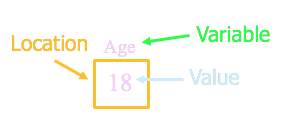
\includegraphics[width=0.5\textwidth]{../../../Data301/Irenes_301_Slides/04VBA/img/Variable.png}$ \\
\begin{alert}
{IMPORTANT:} The \emph{value} at a location can change.% using initialization or assignment.
\end{alert}
\end{itemize}
\end{frame}


\begin{frame}[fragile]{}
\begin{itemize}
\item Notice when you assign something to an object, \R does not automatically print the result to the the screen.
\item For that reason, when we save output to a variable, we will have to call the varaible name or use a print statment to see our result
\end{itemize}
\begin{knitrout}\footnotesize
\definecolor{shadecolor}{rgb}{0.969, 0.969, 0.969}\color{fgcolor}\begin{kframe}
\begin{alltt}
\hlnum{2} \hlopt{+} \hlnum{3}
\end{alltt}
\begin{verbatim}
## [1] 5
\end{verbatim}
\begin{alltt}
\hlstd{x} \hlkwb{=} \hlnum{2}\hlopt{+}\hlnum{3}
\hlstd{x}
\end{alltt}
\begin{verbatim}
## [1] 5
\end{verbatim}
\begin{alltt}
\hlcom{# another alternative:}
\hlstd{(x} \hlkwb{=} \hlnum{2}\hlopt{+}\hlnum{3}\hlstd{)}
\end{alltt}
\begin{verbatim}
## [1] 5
\end{verbatim}
\end{kframe}
\end{knitrout}
\end{frame}


% \section{Data types}
% \begin{frame}[fragile]{Classes}
% \begin{itemize}
% \item There are many \textit{classes} in R and each have different rules.
% \item You can even create your own class in \R (but this is beyond the scope of this course)
% \item The function {\tt class(x)} will tell you what kind of object {\tt x} is.
% \end{itemize}
% \end{frame}




\begin{frame}[fragile]{Data types}
\begin{itemize}
\item Here's a list of some important data types used in R:
 \begin{enumerate}
\item Integer (Whole Numbers)
\item Numeric (Real Numbers)
\item Character
\item Logical (True / False)
\item Factor
\item Complex (we don't focus on this type)
 \end{enumerate}
\end{itemize}
\end{frame}


\begin{frame}[fragile]{Numeric and Integer}
\begin{itemize}
\item \R will automatically assign the type to a variable once declared. %Notice that integers
\item Often the default storage of numbers in \R is in as numeric.
\item To force a variable to be an interger, we need to use the {\tt as.integer()} function, or use the  ``L'' suffix.
\end{itemize}
\end{frame}


\begin{frame}[fragile]{Numeric and Integer}
\begin{knitrout}\footnotesize
\definecolor{shadecolor}{rgb}{0.969, 0.969, 0.969}\color{fgcolor}\begin{kframe}
\begin{alltt}
\hlstd{numobj} \hlkwb{=} \hlnum{2} \hlcom{# numeric (not integer)}
\hlkwd{as.integer}\hlstd{(numobj)} \hlcom{# integer}
\end{alltt}
\begin{verbatim}
## [1] 2
\end{verbatim}
\begin{alltt}
\hlstd{intobj} \hlkwb{=} \hlnum{2L} \hlcom{# integer }
\end{alltt}
\end{kframe}
\end{knitrout}

\end{frame}

\begin{frame}[fragile]{Character}
\begin{itemize}
\item A single letter or string of characters will be recorded as a {\tt character} object. 
\item  You can use double quotes or single quotes for all of these specifications (just be consistent)
\begin{knitrout}\footnotesize
\definecolor{shadecolor}{rgb}{0.969, 0.969, 0.969}\color{fgcolor}\begin{kframe}
\begin{alltt}
\hlcom{# note our usage of quotes }
\hlstd{charobj} \hlkwb{=} \hlstr{"s"}
\hlstd{strobj} \hlkwb{=} \hlstr{'string'}
\hlcom{# badobj = "str' # unmatched quotes = bad}
\end{alltt}
\end{kframe}
\end{knitrout}
\end{itemize}
\end{frame}

\begin{frame}[fragile]{Aside}{Auto-complete}
Notice that \R trys to help us out by autocompleting our quotes (i.e. when we type one quotation/parenthesis the closing one will appear automatically.  If you don't like this feature, you can turn it off (but I suggest you keep it!)
\end{frame}


\begin{frame}[fragile]{Character}
We can also treat numbers as characters:
\begin{knitrout}\footnotesize
\definecolor{shadecolor}{rgb}{0.969, 0.969, 0.969}\color{fgcolor}\begin{kframe}
\begin{alltt}
\hlstd{x} \hlkwb{=} \hlkwd{c}\hlstd{(}\hlnum{1}\hlstd{,}\hlnum{2}\hlstd{,}\hlnum{3}\hlstd{)}
\hlstd{x}
\end{alltt}
\begin{verbatim}
## [1] 1 2 3
\end{verbatim}
\begin{alltt}
\hlstd{x} \hlkwb{=} \hlkwd{as.character}\hlstd{(x)}
\hlstd{x} \hlcom{# notice the quotes in the output}
\end{alltt}
\begin{verbatim}
## [1] "1" "2" "3"
\end{verbatim}
\begin{alltt}
\hlcom{# PS - To change back to numeric use:}
\hlstd{x} \hlkwb{=} \hlkwd{as.numeric}\hlstd{(x)}
\hlstd{x} \hlcom{# no more quotes}
\end{alltt}
\begin{verbatim}
## [1] 1 2 3
\end{verbatim}
\end{kframe}
\end{knitrout}

\end{frame}


\begin{frame}[fragile]{Logical}
In \R, \texttt{T} and \texttt{F} are reserved for logicals (i.e. True/False objects) and \R reads \texttt{T} the same as \texttt{TRUE} or \texttt{F} the same as \texttt{FALSE}. %Inside of
\begin{knitrout}\footnotesize
\definecolor{shadecolor}{rgb}{0.969, 0.969, 0.969}\color{fgcolor}\begin{kframe}
\begin{alltt}
\hlstd{x} \hlkwb{=} \hlkwd{c}\hlstd{(T,} \hlnum{FALSE}\hlstd{,}\hlnum{TRUE}\hlstd{, F)} \hlcom{# notice we don't use quotes}
\hlstd{x}
\end{alltt}
\begin{verbatim}
## [1]  TRUE FALSE  TRUE FALSE
\end{verbatim}
\end{kframe}
\end{knitrout}
\end{frame}


\begin{frame}[fragile]{Logical}
\begin{itemize}
\item Oftentimes, True and False conditions are coded as 0 and 1s.  To covert them to logical, use {\tt as.logical()}. %Similar functions are available for the other data types; namely, {\tt as.numeric}.
\begin{knitrout}\footnotesize
\definecolor{shadecolor}{rgb}{0.969, 0.969, 0.969}\color{fgcolor}\begin{kframe}
\begin{alltt}
\hlstd{x} \hlkwb{=} \hlkwd{c}\hlstd{(}\hlnum{0}\hlstd{,}\hlnum{1}\hlstd{,}\hlnum{1}\hlstd{,}\hlnum{0}\hlstd{,}\hlnum{0}\hlstd{,}\hlnum{0}\hlstd{,}\hlnum{1}\hlstd{,}\hlnum{0}\hlstd{,}\hlnum{0}\hlstd{,}\hlnum{1}\hlstd{,}\hlnum{1}\hlstd{)}
\hlkwd{class}\hlstd{(x)}
\end{alltt}
\begin{verbatim}
## [1] "numeric"
\end{verbatim}
\begin{alltt}
\hlstd{x} \hlkwb{=} \hlkwd{as.logical}\hlstd{(x)}
\hlkwd{class}\hlstd{(x)}
\end{alltt}
\begin{verbatim}
## [1] "logical"
\end{verbatim}
\end{kframe}
\end{knitrout}
\end{itemize}
\end{frame}


\begin{frame}[fragile]{Factor}
\begin{itemize}
\item If you want a variable to be a factor type (so that different symbols are regarded as a level), use \texttt{var=factor(var)}.
\begin{knitrout}\footnotesize
\definecolor{shadecolor}{rgb}{0.969, 0.969, 0.969}\color{fgcolor}\begin{kframe}
\begin{alltt}
\hlstd{notfactor} \hlkwb{=} \hlkwd{c}\hlstd{(}\hlstr{"H"}\hlstd{,}\hlstr{"M"}\hlstd{,} \hlstr{"M"}\hlstd{,} \hlstr{"L"}\hlstd{,} \hlstr{"H"}\hlstd{)}
\hlstd{notfactor}
\end{alltt}
\begin{verbatim}
## [1] "H" "M" "M" "L" "H"
\end{verbatim}
\begin{alltt}
\hlstd{fvec} \hlkwb{=} \hlkwd{factor}\hlstd{(notfactor)}
\hlstd{fvec}
\end{alltt}
\begin{verbatim}
## [1] H M M L H
## Levels: H L M
\end{verbatim}
\end{kframe}
\end{knitrout}
\end{itemize}
\end{frame}

% factor(x, levels=c(100, 200, 400, 500), ordered=TRUE) Add this
% https://www.r-exercises.com/2015/12/28/factor-exercises/


%% If z <- factor(c("p", "q", "p", "r", "q")) and levels of z are "p", "q" ,"r", write an R expression that will change the level "p" to "w" so that z is equal to: "w", "q" , "w", "r" , "q".
% z <- factor(c("p", "q", "p", "r", "q"))
% levels(z)[1] <- "w"

%Let x <- data.frame(q=c(2, 4, 6), p=c("a", "b", "c")). Write an R statement that will replace levels a, b, c with labels "fertiliser1", "fertliser2", "fertiliser3".
% x <- data.frame(q=c(2, 4, 6), p=c("a", "b", "c"))
% x$p <- factor(x$p, levels=c("a", "b", "c"), labels=c("fertiliser1", "fertiliser2", "fertiliser3"))


\begin{frame}[fragile]{Factor}
\begin{itemize}
\item 
We also have the option to specify the labels to something more meaningful:
\begin{knitrout}\footnotesize
\definecolor{shadecolor}{rgb}{0.969, 0.969, 0.969}\color{fgcolor}\begin{kframe}
\begin{alltt}
\hlstd{fvec} \hlkwb{=} \hlkwd{factor}\hlstd{(}\hlkwc{x}\hlstd{=notfactor,} \hlkwc{labels}\hlstd{=}\hlkwd{c}\hlstd{(}\hlstr{"High"}\hlstd{,}\hlstr{"Medium"}\hlstd{,}\hlstr{"Low"}\hlstd{))}
\hlstd{fvec}
\end{alltt}
\begin{verbatim}
## [1] High   Low    Low    Medium High  
## Levels: High Medium Low
\end{verbatim}
\end{kframe}
\end{knitrout}
\end{itemize}
\end{frame}

\begin{frame}[fragile]{Aside}{Notation}
\begin{itemize}
\item We say that {\tt factor()} is a \define{function} for which we have specified two \define{arguments} (having argument names: {\tt from}, {\tt x} and {\tt labels}).
\item You can access the help file to see the details of this function using {\tt ?factor}
\item Notice that is has other (optional) arguments that we haven't specified.  
\end{itemize}
\end{frame}


\begin{frame}[fragile]{Factor}
\begin{itemize}
\item The case my also arise that we need to specify levels not seen in the data set.  In that case we can specify the {\tt levels} argument:
\item Using {\tt letters} a built in vector containing the 26 letters of the alphabet;
\begin{knitrout}\footnotesize
\definecolor{shadecolor}{rgb}{0.969, 0.969, 0.969}\color{fgcolor}\begin{kframe}
\begin{alltt}
\hlstd{x} \hlkwb{=} \hlkwd{c}\hlstd{(}\hlstr{"o"}\hlstd{,}\hlstr{"q"}\hlstd{,}\hlstr{"h"}\hlstd{,}\hlstr{"n"}\hlstd{,}\hlstr{"s"}\hlstd{,}\hlstr{"b"}\hlstd{,}\hlstr{"u"}\hlstd{,}\hlstr{"d"}\hlstd{,}\hlstr{"p"}\hlstd{,}\hlstr{"r"}\hlstd{)}
\hlstd{xlist} \hlkwb{=} \hlkwd{factor}\hlstd{(x,} \hlkwc{levels}\hlstd{=letters)}
\hlkwd{table}\hlstd{(xlist)}
\end{alltt}
\begin{verbatim}
## xlist
## a b c d e f g h i j k l m n o p q r s t u v w x y z 
## 0 1 0 1 0 0 0 1 0 0 0 0 0 1 1 1 1 1 1 0 1 0 0 0 0 0
\end{verbatim}
\end{kframe}
\end{knitrout}
\end{itemize}
\end{frame}


\begin{frame}[fragile]{Aside}{Built-in Constants}
\begin{itemize}
\item On the previous slide we used the built-in constant {\tt letters}
\item Other build in constants include:
\begin{itemize}
\item {\tt LETTERS} (capital letters)
\item {\tt month.name} (eg. ``January", ``February", etc..)
\item {\tt month.abb} (eg. ``Jan", ``Feb", etc..)
\item {\tt pi} 3.141593
\end{itemize}
\end{itemize}
\end{frame}



\begin{frame}[fragile]{Data structures}
\begin{itemize}
\item R has a wide variety of data structures including:
\begin{itemize}
\item scalars
\item vectors (numerical, character, logical)
\item matrices
\item data frames, and
\item lists.
\end{itemize}
\end{itemize}
\end{frame}



\begin{frame}[fragile]{Vectors}
\begin{itemize}
\item A vector is the most basic data structure in \R and can be of two types:
\begin{itemize}
\item atomic vectors
\item lists
\end{itemize}
\item As we did in the examples above, you can create a vector using \texttt{c} (see {\tt ?c} for more details on this \textit{combine} function)
\end{itemize}
\end{frame}


\begin{frame}[fragile]{Vectors}
Atomic Vectors can be vectors characters, logical, integers or numeric.
\begin{knitrout}\footnotesize
\definecolor{shadecolor}{rgb}{0.969, 0.969, 0.969}\color{fgcolor}\begin{kframe}
\begin{alltt}
\hlcom{# example of a numeric vector:}
\hlstd{y}\hlkwb{=}\hlkwd{c}\hlstd{(}\hlnum{2}\hlstd{,}\hlnum{3}\hlstd{,}\hlnum{0}\hlstd{,}\hlnum{3}\hlstd{,}\hlnum{1}\hlstd{,}\hlnum{0}\hlstd{,}\hlnum{0}\hlstd{,}\hlnum{1}\hlstd{)}
\hlcom{# example of a character vector:}
\hlstd{letters}\hlkwb{<-}\hlkwd{c}\hlstd{(}\hlstr{'A'}\hlstd{,}\hlstr{'B'}\hlstd{,}\hlstr{'C'}\hlstd{)}
\hlcom{# example of a logical vector:}
\hlstd{lvec} \hlkwb{<-} \hlkwd{c}\hlstd{(}\hlnum{TRUE}\hlstd{,} \hlnum{FALSE}\hlstd{,} \hlnum{FALSE}\hlstd{)}
\end{alltt}
\end{kframe}
\end{knitrout}
\end{frame}


\begin{frame}[fragile]{Vectors}
Numeric vectors can be created a number of different ways. 
\begin{knitrout}\footnotesize
\definecolor{shadecolor}{rgb}{0.969, 0.969, 0.969}\color{fgcolor}\begin{kframe}
\begin{alltt}
\hlcom{# Ceate a vector of size 10, where each element is a 2:}
\hlstd{y}\hlkwb{=}\hlkwd{rep}\hlstd{(}\hlnum{2}\hlstd{,}\hlnum{10}\hlstd{)}
\hlcom{# This specifies a sequence of integers:}
\hlstd{y}\hlkwb{=}\hlnum{3}\hlopt{:}\hlnum{12}
\hlcom{#This specifies a sequence of real numbers:}
\hlstd{z}\hlkwb{=}\hlkwd{seq}\hlstd{(}\hlkwc{from}\hlstd{=}\hlnum{1}\hlstd{,}\hlkwc{to}\hlstd{=}\hlnum{2}\hlstd{,}\hlkwc{by}\hlstd{=}\hlnum{0.1}\hlstd{)}
\hlcom{#This specifies a sequence of real numbers:}
\hlstd{z}\hlkwb{=}\hlkwd{seq}\hlstd{(}\hlkwc{from}\hlstd{=}\hlnum{2}\hlstd{,}\hlkwc{to}\hlstd{=}\hlnum{1}\hlstd{,}\hlkwc{by}\hlstd{=}\hlopt{-}\hlnum{0.1}\hlstd{)}
\end{alltt}
\end{kframe}
\end{knitrout}
\end{frame}


\begin{frame}[fragile]{Aside}{Notation}
\begin{itemize}
\item We say that {\tt seq()} is a \define{function} for which we have specified three \define{arguments} (having argument names: {\tt from}, {\tt to} and {\tt by}).
\item Assuming we are putting the values in the correct order, you do not need to specify the argument names explicitly.
\begin{knitrout}\footnotesize
\definecolor{shadecolor}{rgb}{0.969, 0.969, 0.969}\color{fgcolor}\begin{kframe}
\begin{alltt}
\hlkwd{seq}\hlstd{(}\hlnum{1}\hlstd{,}\hlnum{2}\hlstd{,}\hlnum{0.1}\hlstd{)} \hlcom{# same as seq(from=1,to=2,by=0.1)}
\end{alltt}
\begin{verbatim}
##  [1] 1.0 1.1 1.2 1.3 1.4 1.5 1.6 1.7 1.8 1.9 2.0
\end{verbatim}
\begin{alltt}
\hlcom{# if we want to specify arguments out of order, }
\hlcom{# we HAVE to include argument names:}
\hlkwd{seq}\hlstd{(}\hlkwc{by}\hlstd{=}\hlnum{0.1}\hlstd{,} \hlkwc{to}\hlstd{=}\hlnum{2}\hlstd{,} \hlkwc{from}\hlstd{=}\hlnum{1}\hlstd{)} \hlcom{# arguments in green}
\end{alltt}
\begin{verbatim}
##  [1] 1.0 1.1 1.2 1.3 1.4 1.5 1.6 1.7 1.8 1.9 2.0
\end{verbatim}
\end{kframe}
\end{knitrout}
\end{itemize}
\end{frame}




\begin{frame}[fragile,label={seed}]{Vectors}
Numeric vectors can be created a number of different ways. 
\begin{knitrout}\footnotesize
\definecolor{shadecolor}{rgb}{0.969, 0.969, 0.969}\color{fgcolor}\begin{kframe}
\begin{alltt}
\hlcom{# Ceates a vector of size 10, of random numbers between 0 and 1}
\hlstd{y}\hlkwb{=}\hlkwd{runif}\hlstd{(}\hlnum{10}\hlstd{)}
\hlcom{# Creates a vector of size 3 sampled from x without replacement}
\hlkwd{set.seed}\hlstd{(}\hlnum{4758}\hlstd{)}
\hlstd{(y}\hlkwb{=}\hlkwd{sample}\hlstd{(}\hlkwc{x}\hlstd{=}\hlkwd{c}\hlstd{(}\hlnum{1}\hlstd{,}\hlnum{2}\hlstd{,}\hlnum{3}\hlstd{),} \hlkwc{size}\hlstd{=}\hlnum{3}\hlstd{))}
\end{alltt}
\begin{verbatim}
## [1] 3 2 1
\end{verbatim}
\begin{alltt}
\hlcom{# Creates a vector of size 3 sampled from x with replacement}
\hlstd{(y}\hlkwb{=}\hlkwd{sample}\hlstd{(}\hlkwc{x}\hlstd{=}\hlkwd{c}\hlstd{(}\hlnum{1}\hlstd{,}\hlnum{2}\hlstd{,}\hlnum{3}\hlstd{),} \hlkwc{size}\hlstd{=}\hlnum{3}\hlstd{,} \hlkwc{replace}\hlstd{=}\hlnum{TRUE}\hlstd{))}
\end{alltt}
\begin{verbatim}
## [1] 3 2 2
\end{verbatim}
\end{kframe}
\end{knitrout}
\end{frame}

\begin{frame}[fragile]{Vectors}
We can also create empty vectors
\begin{knitrout}\footnotesize
\definecolor{shadecolor}{rgb}{0.969, 0.969, 0.969}\color{fgcolor}\begin{kframe}
\begin{alltt}
\hlstd{x} \hlkwb{<-} \hlkwd{vector}\hlstd{()} \hlcom{# defaults to logical (FALSE)}
\hlstd{x} \hlkwb{<-} \hlkwd{vector}\hlstd{(}\hlkwc{length} \hlstd{=} \hlnum{10}\hlstd{)} \hlcom{# defaults to logical vec of FALSES}
\hlstd{x} \hlkwb{<-} \hlkwd{vector}\hlstd{(}\hlstr{"character"}\hlstd{,} \hlkwc{length} \hlstd{=} \hlnum{10}\hlstd{)}
\hlstd{x} \hlkwb{<-} \hlkwd{vector}\hlstd{(}\hlstr{"numeric"}\hlstd{,}   \hlkwc{length} \hlstd{=} \hlnum{10}\hlstd{)}
\hlstd{x} \hlkwb{<-} \hlkwd{vector}\hlstd{(}\hlstr{"integer"}\hlstd{,}   \hlkwc{length} \hlstd{=} \hlnum{10}\hlstd{)}
\hlstd{x} \hlkwb{<-} \hlkwd{vector}\hlstd{(}\hlstr{"logical"}\hlstd{,}   \hlkwc{length} \hlstd{=} \hlnum{10}\hlstd{)}
\end{alltt}
\end{kframe}
\end{knitrout}
\end{frame}


\begin{frame}[fragile]{Seed}
\begin{itemize}
\item Notice that I use {\tt set.seed(4758)} on \hyperlink{seed}{\beamerbutton{slide}} \ref{seed}.
\item This was created so that when you run the same exact code on our computer, you will obtain the same `random' numbers.
\item A random seed is a number used to initialize a pseudorandom number generator.
\item Without going into to much detail, setting a seed using {\tt set.seed} will yield same `random` results every time.
\end{itemize}
\end{frame}


\begin{frame}[fragile]{}
\begin{knitrout}\footnotesize
\definecolor{shadecolor}{rgb}{0.969, 0.969, 0.969}\color{fgcolor}\begin{kframe}
\begin{alltt}
\hlkwd{set.seed}\hlstd{(}\hlnum{4444}\hlstd{)}
\hlkwd{runif}\hlstd{(}\hlnum{1}\hlstd{)}
\end{alltt}
\begin{verbatim}
## [1] 0.9849711
\end{verbatim}
\begin{alltt}
\hlkwd{set.seed}\hlstd{(}\hlnum{4444}\hlstd{)}
\hlkwd{runif}\hlstd{(}\hlnum{1}\hlstd{)}
\end{alltt}
\begin{verbatim}
## [1] 0.9849711
\end{verbatim}
\begin{alltt}
\hlkwd{runif}\hlstd{(}\hlnum{1}\hlstd{)}
\end{alltt}
\begin{verbatim}
## [1] 0.1085671
\end{verbatim}
\end{kframe}
\end{knitrout}
\end{frame}


\begin{frame}[fragile]{Scalars}
Scalars are just vectors of length 1.  To check the length of any vector use {\tt length()}
\begin{knitrout}\footnotesize
\definecolor{shadecolor}{rgb}{0.969, 0.969, 0.969}\color{fgcolor}\begin{kframe}
\begin{alltt}
\hlstd{x} \hlkwb{=} \hlnum{4}
\hlkwd{length}\hlstd{(x)}
\end{alltt}
\begin{verbatim}
## [1] 1
\end{verbatim}
\begin{alltt}
\hlstd{y}\hlkwb{=}\hlkwd{c}\hlstd{(}\hlnum{2}\hlstd{,}\hlnum{3}\hlstd{,}\hlnum{0}\hlstd{,}\hlnum{3}\hlstd{,}\hlnum{1}\hlstd{,}\hlnum{0}\hlstd{,}\hlnum{0}\hlstd{,}\hlnum{1}\hlstd{)}
\hlkwd{length}\hlstd{(y)}
\end{alltt}
\begin{verbatim}
## [1] 8
\end{verbatim}
\end{kframe}
\end{knitrout}
\end{frame}

\begin{frame}[fragile]{Indexing Vectors}
To index an element from a vector, use single square brackets
\begin{knitrout}\footnotesize
\definecolor{shadecolor}{rgb}{0.969, 0.969, 0.969}\color{fgcolor}\begin{kframe}
\begin{alltt}
\hlstd{z} \hlkwb{=} \hlkwd{c}\hlstd{(}\hlstr{"apples"}\hlstd{,}\hlstr{"bananas"}\hlstd{,}\hlstr{"oranges"}\hlstd{,} \hlstr{"pineapples"}\hlstd{)}
\hlstd{z[}\hlnum{1}\hlstd{]}
\end{alltt}
\begin{verbatim}
## [1] "apples"
\end{verbatim}
\begin{alltt}
\hlstd{z[}\hlnum{2}\hlopt{:}\hlnum{3}\hlstd{]}
\end{alltt}
\begin{verbatim}
## [1] "bananas" "oranges"
\end{verbatim}
\begin{alltt}
\hlstd{z[}\hlkwd{c}\hlstd{(}\hlnum{4}\hlstd{,}\hlnum{2}\hlstd{)]}
\end{alltt}
\begin{verbatim}
## [1] "pineapples" "bananas"
\end{verbatim}
\begin{alltt}
\hlstd{z[}\hlopt{-}\hlnum{1}\hlstd{]}
\end{alltt}
\begin{verbatim}
## [1] "bananas"    "oranges"    "pineapples"
\end{verbatim}
\end{kframe}
\end{knitrout}
\end{frame}


\begin{frame}[fragile]{}
We have the option of including names for our vector elements.
\begin{knitrout}\footnotesize
\definecolor{shadecolor}{rgb}{0.969, 0.969, 0.969}\color{fgcolor}\begin{kframe}
\begin{alltt}
\hlstd{z} \hlkwb{=} \hlkwd{c}\hlstd{(}\hlnum{123456}\hlstd{,} \hlnum{25}\hlstd{,} \hlnum{2019}\hlstd{);} \hlkwd{names}\hlstd{(z)} \hlkwb{<-} \hlkwd{c}\hlstd{(}\hlstr{"studentID"}\hlstd{,}\hlstr{"age"}\hlstd{,}\hlstr{"year"}\hlstd{)}
\hlstd{z[}\hlstr{"studentID"}\hlstd{]} \hlcom{# same as z[1]}
\end{alltt}
\begin{verbatim}
## studentID 
##    123456
\end{verbatim}
\begin{alltt}
\hlstd{z[}\hlkwd{c}\hlstd{(}\hlstr{"age, year"}\hlstd{)]} \hlcom{# wont work like z[c(2,3)]}
\end{alltt}
\begin{verbatim}
## <NA> 
##   NA
\end{verbatim}
\begin{alltt}
\hlstd{z[}\hlkwd{c}\hlstd{(}\hlnum{FALSE}\hlstd{,} \hlnum{TRUE}\hlstd{,} \hlnum{TRUE}\hlstd{)]} \hlcom{# will work }
\end{alltt}
\begin{verbatim}
##  age year 
##   25 2019
\end{verbatim}
\begin{alltt}
\hlstd{z[}\hlopt{-}\hlstr{"year"}\hlstd{]} \hlcom{# wont work like z[-3]}
\end{alltt}


{\ttfamily\noindent\bfseries\color{errorcolor}{\#\# Error in -"{}year"{}: invalid argument to unary operator}}\end{kframe}
\end{knitrout}
\end{frame}

\begin{frame}[fragile]{}
To add a new element/delete/replace an element:
\begin{knitrout}\footnotesize
\definecolor{shadecolor}{rgb}{0.969, 0.969, 0.969}\color{fgcolor}\begin{kframe}
\begin{alltt}
\hlstd{z} \hlkwb{=} \hlkwd{c}\hlstd{(}\hlstr{"first"}\hlstd{,}\hlstr{"second"}\hlstd{,}\hlstr{"third"}\hlstd{,} \hlstr{"fourth"}\hlstd{)}
\hlcom{# adds a fith element and replaces the second}
\hlstd{z[}\hlnum{5}\hlstd{]} \hlkwb{=} \hlstr{"fifth"}\hlstd{;  z[}\hlnum{2}\hlstd{]} \hlkwb{=} \hlstr{"2nd"}
\hlstd{z}
\end{alltt}
\begin{verbatim}
## [1] "first"  "2nd"    "third"  "fourth" "fifth"
\end{verbatim}
\begin{alltt}
\hlcom{#removes the second element}
\hlstd{(z} \hlkwb{=} \hlstd{z[}\hlopt{-}\hlnum{2}\hlstd{])}
\end{alltt}
\begin{verbatim}
## [1] "first"  "third"  "fourth" "fifth"
\end{verbatim}
\end{kframe}
\end{knitrout}
\end{frame}

\begin{frame}[fragile]{}
Notice what happens if we add a 10th element to z (without specifying elements 6--9):
\begin{knitrout}\footnotesize
\definecolor{shadecolor}{rgb}{0.969, 0.969, 0.969}\color{fgcolor}\begin{kframe}
\begin{alltt}
\hlstd{z[}\hlnum{10}\hlstd{]} \hlkwb{=} \hlstr{"tenth"}
\hlstd{z}
\end{alltt}
\begin{verbatim}
##  [1] "first"  "third"  "fourth" "fifth"  NA       NA       NA      
##  [8] NA       NA       "tenth"
\end{verbatim}
\end{kframe}
\end{knitrout}
\end{frame}

\begin{frame}[fragile]{}
We can also add new named elements
\begin{knitrout}\footnotesize
\definecolor{shadecolor}{rgb}{0.969, 0.969, 0.969}\color{fgcolor}\begin{kframe}
\begin{alltt}
\hlstd{z} \hlkwb{=} \hlkwd{c}\hlstd{(}\hlnum{123456}\hlstd{,} \hlnum{25}\hlstd{,} \hlnum{2019}\hlstd{);} \hlkwd{names}\hlstd{(z)} \hlkwb{<-} \hlkwd{c}\hlstd{(}\hlstr{"studentID"}\hlstd{,}\hlstr{"age"}\hlstd{,}\hlstr{"year"}\hlstd{)}
\hlcom{# adds a forth element with the students major}
\hlstd{z[}\hlstr{"major"}\hlstd{]} \hlkwb{=} \hlstr{"COSC"}
\hlstd{z}
\end{alltt}
\begin{verbatim}
## studentID       age      year     major 
##  "123456"      "25"    "2019"    "COSC"
\end{verbatim}
\end{kframe}
\end{knitrout}
Notice how the addition of this forth element cuase the vector to change to a vector of characters! More on this \hyperlink{coercion}{later}
\end{frame}


\begin{frame}[fragile]{Basic Operations for Vectors}
We can also perform basic operations on vectors:
\begin{center}
\begin{tabular}{ll}
Operation & Command \\\hline 
natural log & \verb!log(x)!\\
Exponent & \verb!exp(x)!\\
Log base 10 & \verb!log10(x)!\\
Absolute value & \verb!abs(x)!\\
Square root & \verb!sqrt(x)!\\
Sum & \verb!sum(x)!\\
Number of elements in $x$  & \verb!length(x)!\\
\end{tabular}
\end{center}
\end{frame}


\begin{frame}[fragile]{}
\begin{center}
\begin{tabular}{ll}
Unique elements of $x$ & \verb!unique(x)!\\
Mean & \verb!mean(x)!\\
Variance & \verb!var(x)!\\
Standard Deviation & \verb!sd(x)!\\
Minimum value & \verb!min(x)!\\
Maximum value & \verb!max(x)!\\
Smallest and largest values  & \verb!range(x)!\\
median & \verb!median(x)!\\
Basic statistical summary & \verb!summary(x)!\\
Sort & \verb!sort(x)!\\
\end{tabular}
\end{center}
\end{frame}


\begin{frame}[fragile]{}


\begin{knitrout}\footnotesize
\definecolor{shadecolor}{rgb}{0.969, 0.969, 0.969}\color{fgcolor}\begin{kframe}
\begin{alltt}
\hlstd{(y}\hlkwb{=} \hlkwd{sample}\hlstd{(}\hlnum{1}\hlopt{:}\hlnum{20}\hlstd{,} \hlnum{9}\hlstd{))} \hlcom{# samples 9 random numbers from 1 to 20}
\end{alltt}
\begin{verbatim}
## [1]  6 15  8 16 17  1 18 12  7
\end{verbatim}
\begin{alltt}
\hlcom{# multiplies each element by 2}
\hlnum{2}\hlopt{*}\hlstd{y}
\end{alltt}
\begin{verbatim}
## [1] 12 30 16 32 34  2 36 24 14
\end{verbatim}
\begin{alltt}
\hlkwd{sort}\hlstd{(y)}
\end{alltt}
\begin{verbatim}
## [1]  1  6  7  8 12 15 16 17 18
\end{verbatim}
\begin{alltt}
\hlkwd{sort}\hlstd{(y,} \hlkwc{decreasing} \hlstd{=} \hlnum{TRUE}\hlstd{)}
\end{alltt}
\begin{verbatim}
## [1] 18 17 16 15 12  8  7  6  1
\end{verbatim}
\begin{alltt}
\hlkwd{summary}\hlstd{(y)}
\end{alltt}
\begin{verbatim}
##    Min. 1st Qu.  Median    Mean 3rd Qu.    Max. 
##    1.00    7.00   12.00   11.11   16.00   18.00
\end{verbatim}
\end{kframe}
\end{knitrout}
\end{frame}

\begin{frame}[fragile]{coercion}\label{coercion}
\begin{itemize}
\item By \textit{atomic vectors} we mean they can only take on one data type. 
\item If we specify more than one type in a single vector, \R will  convert the mixed types to a single type which it deems most appropriate.
\item The coercion will move towards the one that's easiest to coerce to.
\item You can coerce vectors explicitly using the {\tt as.<}\textit{class}{\tt>} (eg. {\tt as.numeric}, {\tt as.character}, etc. )
\end{itemize}
\end{frame}

\begin{frame}[fragile]{}
\begin{knitrout}\footnotesize
\definecolor{shadecolor}{rgb}{0.969, 0.969, 0.969}\color{fgcolor}\begin{kframe}
\begin{alltt}
\hlstd{(x} \hlkwb{=} \hlkwd{c}\hlstd{(}\hlstr{"apple"}\hlstd{,} \hlnum{2}\hlstd{,} \hlnum{TRUE}\hlstd{))} \hlcom{# converts all to character}
\end{alltt}
\begin{verbatim}
## [1] "apple" "2"     "TRUE"
\end{verbatim}
\begin{alltt}
\hlstd{(x} \hlkwb{=} \hlkwd{c}\hlstd{(}\hlnum{TRUE}\hlstd{,} \hlnum{4}\hlstd{))} \hlcom{# converts all to numeric}
\end{alltt}
\begin{verbatim}
## [1] 1 4
\end{verbatim}
\begin{alltt}
\hlstd{(x} \hlkwb{=} \hlkwd{c}\hlstd{(}\hlnum{2L}\hlstd{,} \hlopt{-}\hlnum{1.3}\hlstd{))} \hlcom{# converts to numeric}
\end{alltt}
\begin{verbatim}
## [1]  2.0 -1.3
\end{verbatim}
\begin{alltt}
\hlstd{(x} \hlkwb{=} \hlkwd{c}\hlstd{(}\hlnum{TRUE}\hlstd{,} \hlnum{0}\hlstd{,} \hlnum{1}\hlstd{,} \hlnum{FALSE}\hlstd{))} \hlcom{# converts all to numeric}
\end{alltt}
\begin{verbatim}
## [1] 1 0 1 0
\end{verbatim}
\begin{alltt}
\hlkwd{as.logical}\hlstd{(}\hlkwc{x} \hlstd{=} \hlkwd{c}\hlstd{(}\hlnum{TRUE}\hlstd{,} \hlnum{0}\hlstd{,} \hlnum{1}\hlstd{,} \hlnum{FALSE}\hlstd{))} \hlcom{# converts to logical}
\end{alltt}
\begin{verbatim}
## [1]  TRUE FALSE  TRUE FALSE
\end{verbatim}
\end{kframe}
\end{knitrout}
\end{frame}

\begin{frame}[fragile]{Matrices}
\begin{itemize}
\item While we can view matrices as column vectors stacked side by side or row vectors stack one on top of another, matrices are really just a vector in \R.
item The main difference between matrices and the vectors discussed in the previous slides is that a matrix has a \define{dimension}. 
\item The dimenions can be found using the {\tt dim()} function. 
\end{itemize}
\end{frame}


\begin{frame}[fragile]{Matrices}
\begin{knitrout}\footnotesize
\definecolor{shadecolor}{rgb}{0.969, 0.969, 0.969}\color{fgcolor}\begin{kframe}
\begin{alltt}
\hlstd{(m} \hlkwb{<-} \hlkwd{matrix}\hlstd{(}\hlnum{1}\hlopt{:}\hlnum{8}\hlstd{,} \hlkwc{nrow} \hlstd{=} \hlnum{2}\hlstd{,} \hlkwc{ncol} \hlstd{=} \hlnum{4}\hlstd{))}
\end{alltt}
\begin{verbatim}
##      [,1] [,2] [,3] [,4]
## [1,]    1    3    5    7
## [2,]    2    4    6    8
\end{verbatim}
\begin{alltt}
\hlkwd{dim}\hlstd{(m)} \hlcom{# gives the number or rows and columns}
\end{alltt}
\begin{verbatim}
## [1] 2 4
\end{verbatim}
\begin{alltt}
\hlkwd{class}\hlstd{(m)}
\end{alltt}
\begin{verbatim}
## [1] "matrix"
\end{verbatim}
\end{kframe}
\end{knitrout}
\end{frame}

\begin{frame}[fragile]{Matrices}
\begin{itemize}
\item By default, matrices are constructed columnwise.  
\item You can always change to row-wise by specifying {\tt byrow=TRUE}
\end{itemize}
\begin{knitrout}\footnotesize
\definecolor{shadecolor}{rgb}{0.969, 0.969, 0.969}\color{fgcolor}\begin{kframe}
\begin{alltt}
\hlstd{(m} \hlkwb{<-} \hlkwd{matrix}\hlstd{(}\hlnum{1}\hlopt{:}\hlnum{6}\hlstd{,} \hlkwc{nrow}\hlstd{=}\hlnum{2}\hlstd{,} \hlkwc{ncol} \hlstd{=}\hlnum{3}\hlstd{))} \hlcom{# fill columnwise}
\end{alltt}
\begin{verbatim}
##      [,1] [,2] [,3]
## [1,]    1    3    5
## [2,]    2    4    6
\end{verbatim}
\begin{alltt}
\hlstd{(m} \hlkwb{<-} \hlkwd{matrix}\hlstd{(}\hlnum{1}\hlopt{:}\hlnum{6}\hlstd{,} \hlkwc{nrow}\hlstd{=}\hlnum{2}\hlstd{,} \hlkwc{ncol} \hlstd{=}\hlnum{3}\hlstd{,} \hlkwc{byrow}\hlstd{=}\hlnum{TRUE}\hlstd{))} \hlcom{#fill row-wise}
\end{alltt}
\begin{verbatim}
##      [,1] [,2] [,3]
## [1,]    1    2    3
## [2,]    4    5    6
\end{verbatim}
\end{kframe}
\end{knitrout}
\end{frame}


\begin{frame}[fragile]{Matrices}
An alternative way of constructing matrices is to use {\tt array()}
\begin{knitrout}\footnotesize
\definecolor{shadecolor}{rgb}{0.969, 0.969, 0.969}\color{fgcolor}\begin{kframe}
\begin{alltt}
\hlkwd{array}\hlstd{(}\hlnum{1}\hlopt{:}\hlnum{6}\hlstd{,} \hlkwc{dim}\hlstd{=}\hlkwd{c}\hlstd{(}\hlnum{2}\hlstd{,}\hlnum{3}\hlstd{))}
\end{alltt}
\begin{verbatim}
##      [,1] [,2] [,3]
## [1,]    1    3    5
## [2,]    2    4    6
\end{verbatim}
\end{kframe}
\end{knitrout}
\end{frame}


\begin{frame}[fragile]{Named Matrices}
We may also choose to name our rows and columns
\begin{knitrout}\footnotesize
\definecolor{shadecolor}{rgb}{0.969, 0.969, 0.969}\color{fgcolor}\begin{kframe}
\begin{alltt}
\hlkwd{rownames}\hlstd{(m)} \hlkwb{=} \hlkwd{c}\hlstd{(}\hlstr{"row1"}\hlstd{,} \hlstr{"row2"}\hlstd{)}
\hlkwd{colnames}\hlstd{(m)} \hlkwb{=} \hlkwd{c}\hlstd{(}\hlstr{"col1"}\hlstd{,} \hlstr{"col2"}\hlstd{,} \hlstr{"col3"}\hlstd{)}
\hlstd{m}
\end{alltt}
\begin{verbatim}
##      col1 col2 col3
## row1    1    2    3
## row2    4    5    6
\end{verbatim}
\end{kframe}
\end{knitrout}
\end{frame}


\begin{frame}[fragile]{Indexing}
\begin{itemize}
\item To index an element from a matrix, we can again use square brackets, but we need to specify TWO numbers {\tt[row, col]}.
\item  If we want to extract an entire row, we'll leave the {\tt col} field blank (indicating we want all colums).
\item  If we want to extract an entire column, we'll leave the {\tt row} field blank (indicating we want all rows).
\end{itemize}
\end{frame}

\begin{frame}[fragile]{Indexing}
The following extracts a column, row, and cell from matrix {\tt m},
\begin{knitrout}\footnotesize
\definecolor{shadecolor}{rgb}{0.969, 0.969, 0.969}\color{fgcolor}\begin{kframe}
\begin{alltt}
\hlcom{# extract the third column of m}
\hlstd{m[,}\hlnum{3}\hlstd{]}
\end{alltt}
\begin{verbatim}
## row1 row2 
##    3    6
\end{verbatim}
\begin{alltt}
\hlcom{# extract the first row of m}
\hlstd{m[}\hlnum{1}\hlstd{,]}
\end{alltt}
\begin{verbatim}
## col1 col2 col3 
##    1    2    3
\end{verbatim}
\begin{alltt}
\hlcom{# extract the element in the 1st row and 3rd column}
\hlstd{m[}\hlnum{1}\hlstd{,}\hlnum{3}\hlstd{]}
\end{alltt}
\begin{verbatim}
## [1] 3
\end{verbatim}
\end{kframe}
\end{knitrout}
\end{frame}

\begin{frame}[fragile]{}
Alternatively we could call them by name
\begin{knitrout}\footnotesize
\definecolor{shadecolor}{rgb}{0.969, 0.969, 0.969}\color{fgcolor}\begin{kframe}
\begin{alltt}
\hlcom{# extract the third column of m}
\hlstd{m[,}\hlstr{"col3"}\hlstd{]} \hlcom{# same as m[,3]}
\end{alltt}
\begin{verbatim}
## row1 row2 
##    3    6
\end{verbatim}
\begin{alltt}
\hlcom{# extract the first row of m}
\hlstd{m[}\hlstr{"row1"}\hlstd{,]} \hlcom{# same as m[1,]}
\end{alltt}
\begin{verbatim}
## col1 col2 col3 
##    1    2    3
\end{verbatim}
\begin{alltt}
\hlcom{# extract the element in the 1st row and 3rd column}
\hlstd{m[}\hlstr{"row1"}\hlstd{,}\hlstr{"col3"}\hlstd{]} \hlcom{# same as m[1,3]}
\end{alltt}
\begin{verbatim}
## [1] 3
\end{verbatim}
\end{kframe}
\end{knitrout}
\end{frame}


\begin{frame}[fragile]{Indexing}
Note that we can also use one number (tricker this way)
\begin{knitrout}\footnotesize
\definecolor{shadecolor}{rgb}{0.969, 0.969, 0.969}\color{fgcolor}\begin{kframe}
\begin{alltt}
\hlstd{(m} \hlkwb{=} \hlkwd{matrix}\hlstd{(}\hlnum{11}\hlopt{:}\hlnum{4}\hlstd{,} \hlnum{2}\hlstd{,}\hlnum{4}\hlstd{))}
\end{alltt}
\begin{verbatim}
##      [,1] [,2] [,3] [,4]
## [1,]   11    9    7    5
## [2,]   10    8    6    4
\end{verbatim}
\begin{alltt}
\hlstd{m[}\hlnum{8}\hlstd{]} \hlcom{# extracts the 8th element in m}
\end{alltt}
\begin{verbatim}
## [1] 4
\end{verbatim}
\begin{alltt}
\hlstd{(mVector} \hlkwb{=} \hlkwd{as.numeric}\hlstd{(m))}
\end{alltt}
\begin{verbatim}
## [1] 11 10  9  8  7  6  5  4
\end{verbatim}
\begin{alltt}
\hlstd{mVector[}\hlnum{8}\hlstd{]}
\end{alltt}
\begin{verbatim}
## [1] 4
\end{verbatim}
\end{kframe}
\end{knitrout}
\end{frame}

\begin{frame}[fragile]{Indexing}
Like the vectors discussed earlier, matices fall under the atomic vector category and therefore can only store data of one type:
\begin{knitrout}\footnotesize
\definecolor{shadecolor}{rgb}{0.969, 0.969, 0.969}\color{fgcolor}\begin{kframe}
\begin{alltt}
\hlstd{m} \hlkwb{=} \hlkwd{matrix}\hlstd{(}\hlkwd{c}\hlstd{(}\hlstr{"bananas"}\hlstd{,} \hlnum{2}\hlstd{,} \hlnum{TRUE}\hlstd{,} \hlnum{0}\hlstd{),}  \hlkwc{nrow}\hlstd{=}\hlnum{2}\hlstd{,} \hlkwc{ncol}\hlstd{=}\hlnum{2}\hlstd{)}
\hlcom{# notice how all coerce to characters:}
\hlstd{m}
\end{alltt}
\begin{verbatim}
##      [,1]      [,2]  
## [1,] "bananas" "TRUE"
## [2,] "2"       "0"
\end{verbatim}
\end{kframe}
\end{knitrout}
\end{frame}




\begin{frame}[fragile]{lists}
\begin{itemize}
\item
If we want our vector to contain objects of different data types we need to create a list.
\item We can think of lists as a special type of vector that can mix data types and  structures
\end{itemize}
\end{frame}

\begin{frame}[fragile]{}

\begin{knitrout}\scriptsize
\definecolor{shadecolor}{rgb}{0.969, 0.969, 0.969}\color{fgcolor}\begin{kframe}
\begin{alltt}
\hlstd{(x} \hlkwb{=} \hlkwd{list}\hlstd{(}\hlstr{"apple"}\hlstd{,} \hlstr{"banana"}\hlstd{,} \hlnum{2}\hlstd{,} \hlnum{TRUE}\hlstd{,} \hlnum{4}\hlstd{,} \hlstr{"four"}\hlstd{))}
\end{alltt}
\begin{verbatim}
## [[1]]
## [1] "apple"
## 
## [[2]]
## [1] "banana"
## 
## [[3]]
## [1] 2
## 
## [[4]]
## [1] TRUE
## 
## [[5]]
## [1] 4
## 
## [[6]]
## [1] "four"
\end{verbatim}
\end{kframe}
\end{knitrout}
\end{frame}


\begin{frame}[fragile]{lists}
Unlike vectors, the member of a list are accessed using double square brackets:
\begin{knitrout}\footnotesize
\definecolor{shadecolor}{rgb}{0.969, 0.969, 0.969}\color{fgcolor}\begin{kframe}
\begin{alltt}
\hlstd{x[[}\hlnum{1}\hlstd{]]} \hlcom{# first member}
\end{alltt}
\begin{verbatim}
## [1] "apple"
\end{verbatim}
\begin{alltt}
\hlstd{x[[}\hlnum{2}\hlstd{]]} \hlcom{# second member, and so on ...}
\end{alltt}
\begin{verbatim}
## [1] "banana"
\end{verbatim}
\end{kframe}
\end{knitrout}
\end{frame}

\begin{frame}[fragile]{lists}
\begin{itemize}
\item While I have specified each member to be a single word/number/logical, we could also have specified them to be vectors or matrices. 
\item To index the elements within the members of a list we use single square brackets (usually nested after double square brackets)
\end{itemize}
\end{frame}


\begin{frame}[fragile]{lists}
\begin{knitrout}\footnotesize
\definecolor{shadecolor}{rgb}{0.969, 0.969, 0.969}\color{fgcolor}\begin{kframe}
\begin{alltt}
\hlstd{y} \hlkwb{=} \hlkwd{list}\hlstd{(}\hlkwd{c}\hlstd{(}\hlstr{"apples"}\hlstd{,} \hlstr{"banana"}\hlstd{,} \hlstr{"four"}\hlstd{),} \hlkwd{c}\hlstd{(}\hlnum{2}\hlstd{,}\hlnum{4}\hlstd{),} \hlnum{TRUE}\hlstd{)}
\hlstd{y}
\end{alltt}
\begin{verbatim}
## [[1]]
## [1] "apples" "banana" "four"  
## 
## [[2]]
## [1] 2 4
## 
## [[3]]
## [1] TRUE
\end{verbatim}
\end{kframe}
\end{knitrout}
\end{frame}

\begin{frame}[fragile]{lists}
\begin{knitrout}\footnotesize
\definecolor{shadecolor}{rgb}{0.969, 0.969, 0.969}\color{fgcolor}\begin{kframe}
\begin{alltt}
\hlstd{y[[}\hlnum{1}\hlstd{]][}\hlnum{3}\hlstd{]} \hlcom{# the third element of the first member of y}
\end{alltt}
\begin{verbatim}
## [1] "four"
\end{verbatim}
\begin{alltt}
\hlstd{y[[}\hlnum{2}\hlstd{]][}\hlnum{1}\hlstd{]} \hlcom{# the first element of the second member of y}
\end{alltt}
\begin{verbatim}
## [1] 2
\end{verbatim}
\begin{alltt}
\hlstd{y[[}\hlnum{1}\hlstd{]][}\hlnum{4}\hlstd{]} \hlcom{# calling something that does not exist }
\end{alltt}
\begin{verbatim}
## [1] NA
\end{verbatim}
\end{kframe}
\end{knitrout}
\end{frame}

\begin{frame}[fragile]{Named lists}
Alternatively we could have names for our list members
\begin{knitrout}\footnotesize
\definecolor{shadecolor}{rgb}{0.969, 0.969, 0.969}\color{fgcolor}\begin{kframe}
\begin{alltt}
\hlstd{numbers}\hlkwb{=} \hlkwd{c}\hlstd{(}\hlnum{2}\hlstd{,}\hlnum{4}\hlstd{)} \hlcom{# can define the member outside first}
\hlstd{y} \hlkwb{=} \hlkwd{list}\hlstd{(}\hlkwc{words}\hlstd{=}\hlkwd{c}\hlstd{(}\hlstr{"apples"}\hlstd{,} \hlstr{"banana"}\hlstd{,} \hlstr{"four"}\hlstd{),}
         \hlstd{numbers,} \hlkwc{logicals}\hlstd{=}\hlnum{TRUE}\hlstd{)}
\hlstd{y}\hlopt{$}\hlstd{words} \hlcom{# same this as y[[1]]}
\end{alltt}
\begin{verbatim}
## [1] "apples" "banana" "four"
\end{verbatim}
\begin{alltt}
\hlstd{y}\hlopt{$}\hlstd{numbers} \hlcom{# same this as y[[2]]}
\end{alltt}
\begin{verbatim}
## NULL
\end{verbatim}
\begin{alltt}
\hlstd{y}\hlopt{$}\hlstd{logicals} \hlcom{# same this as y[[3]]}
\end{alltt}
\begin{verbatim}
## [1] TRUE
\end{verbatim}
\end{kframe}
\end{knitrout}
\end{frame}


\begin{frame}[fragile]{}
We could also name the list members after they have been assigned
\begin{knitrout}\footnotesize
\definecolor{shadecolor}{rgb}{0.969, 0.969, 0.969}\color{fgcolor}\begin{kframe}
\begin{alltt}
\hlstd{y} \hlkwb{=} \hlkwd{list}\hlstd{(}\hlkwd{c}\hlstd{(}\hlstr{"apples"}\hlstd{,} \hlstr{"banana"}\hlstd{,} \hlstr{"four"}\hlstd{),}
         \hlkwd{c}\hlstd{(}\hlnum{2}\hlstd{,}\hlnum{4}\hlstd{),} \hlnum{TRUE}\hlstd{)}
\hlkwd{names}\hlstd{(y)} \hlkwb{<-} \hlkwd{c}\hlstd{(}\hlstr{"words"}\hlstd{,}\hlstr{"numbers"}\hlstd{,}\hlstr{"logicals"}\hlstd{)}
\hlstd{y}
\end{alltt}
\begin{verbatim}
## $words
## [1] "apples" "banana" "four"  
## 
## $numbers
## [1] 2 4
## 
## $logicals
## [1] TRUE
\end{verbatim}
\end{kframe}
\end{knitrout}
\end{frame}

\begin{frame}[fragile]{lists}
We can index members of lists using the integer index numbers OR their member names (in quotations) 
\begin{knitrout}\footnotesize
\definecolor{shadecolor}{rgb}{0.969, 0.969, 0.969}\color{fgcolor}\begin{kframe}
\begin{alltt}
\hlstd{y}\hlopt{$}\hlstd{words}
\end{alltt}
\begin{verbatim}
## [1] "apples" "banana" "four"
\end{verbatim}
\begin{alltt}
\hlstd{y[[}\hlstr{"words"}\hlstd{]]}
\end{alltt}
\begin{verbatim}
## [1] "apples" "banana" "four"
\end{verbatim}
\begin{alltt}
\hlstd{y[[}\hlnum{4}\hlstd{]]}
\end{alltt}


{\ttfamily\noindent\bfseries\color{errorcolor}{\#\# Error in y[[4]]: subscript out of bounds}}\begin{alltt}
\hlcom{# the following are not valid:}
\hlcom{# y$4 }
\hlcom{# y[[words]]}
\end{alltt}
\end{kframe}
\end{knitrout}
\end{frame}





\begin{frame}[fragile]{lists}
We can modify its content/add new content directly either using {\tt [[]]} with numbers or {\tt \$} with member names. 
\begin{knitrout}\footnotesize
\definecolor{shadecolor}{rgb}{0.969, 0.969, 0.969}\color{fgcolor}\begin{kframe}
\begin{alltt}
\hlstd{y}\hlopt{$}\hlstd{words[}\hlnum{3}\hlstd{]} \hlkwb{=} \hlstr{"oranges"}\hlcom{#replace the 3rd element of the 1st member}
\hlstd{y[[}\hlnum{1}\hlstd{]][}\hlnum{4}\hlstd{]} \hlkwb{=} \hlstr{"pineapples"}\hlcom{#add a 4th element to the 1st member}
\hlstd{y[[}\hlnum{4}\hlstd{]]} \hlkwb{=} \hlkwd{c}\hlstd{(}\hlnum{0}\hlstd{,}\hlnum{1}\hlstd{,}\hlnum{1}\hlstd{,}\hlnum{0}\hlstd{)} \hlcom{# add a forth member to y}
\hlstd{y}\hlopt{$}\hlstr{"fifth"} \hlkwb{=} \hlnum{3}\hlopt{:}\hlnum{12} \hlcom{# add a fifth member to y (named "fifth")}
\end{alltt}
\end{kframe}
\end{knitrout}
\end{frame}



\begin{frame}[fragile]{Data Frames}
\begin{itemize}
\item Data frames are perhaps the most used data structure used in statistics. 
\item Like list, they can store different data types.
\item Futhermore, they can contain  additional attributes such as column and row names. \item When combining vectors in a data frame  all must have the same size (i.e. length).  \item Missing observations will be recorded as \texttt{NA}.
\end{itemize}
\end{frame}

\begin{frame}[fragile]{Data Frames}
Here is an example of how to create a data frame and add to it: 
\begin{knitrout}\footnotesize
\definecolor{shadecolor}{rgb}{0.969, 0.969, 0.969}\color{fgcolor}\begin{kframe}
\begin{alltt}
\hlstd{Person}\hlkwb{=}\hlkwd{c}\hlstd{(}\hlstr{'John'}\hlstd{,} \hlstr{'Jill'}\hlstd{,} \hlstr{'Jack'}\hlstd{)}
\hlstd{Grade}\hlkwb{=}\hlkwd{c}\hlstd{(}\hlstr{'45'}\hlstd{,}\hlstr{'92'}\hlstd{,}\hlstr{'91'}\hlstd{)}
\hlstd{(Lab}\hlkwb{=}\hlkwd{data.frame}\hlstd{(Person, Grade))}
\end{alltt}
\begin{verbatim}
##   Person Grade
## 1   John    45
## 2   Jill    92
## 3   Jack    91
\end{verbatim}
\end{kframe}
\end{knitrout}
\end{frame}

\begin{frame}[fragile]{Data Frames}
Like matrices, we can create column and row names
\begin{knitrout}\footnotesize
\definecolor{shadecolor}{rgb}{0.969, 0.969, 0.969}\color{fgcolor}\begin{kframe}
\begin{alltt}
\hlkwd{colnames}\hlstd{(Lab)} \hlcom{# adopted from the variable names inputed}
\end{alltt}
\begin{verbatim}
## [1] "Person" "Grade"
\end{verbatim}
\begin{alltt}
\hlkwd{rownames}\hlstd{(Lab)} \hlcom{# default to increasing integers}
\end{alltt}
\begin{verbatim}
## [1] "1" "2" "3"
\end{verbatim}
\begin{alltt}
\hlcom{# we could also add row names if we choose}
\hlkwd{rownames}\hlstd{(Lab)} \hlkwb{=} \hlkwd{c}\hlstd{(}\hlstr{"Student1"}\hlstd{,} \hlstr{"Student2"}\hlstd{,} \hlstr{"Student3"}\hlstd{)}
\hlstd{Lab}
\end{alltt}
\begin{verbatim}
##          Person Grade
## Student1   John    45
## Student2   Jill    92
## Student3   Jack    91
\end{verbatim}
\end{kframe}
\end{knitrout}
\end{frame}

\begin{frame}[fragile]{Data Frames}
Unlike matrices, we can extract a column of this data.frame we use the {\tt \$} notation:
\begin{knitrout}\footnotesize
\definecolor{shadecolor}{rgb}{0.969, 0.969, 0.969}\color{fgcolor}\begin{kframe}
\begin{alltt}
\hlstd{Lab}\hlopt{$}\hlstd{Person}
\end{alltt}
\begin{verbatim}
## [1] John Jill Jack
## Levels: Jack Jill John
\end{verbatim}
\begin{alltt}
\hlstd{Lab}\hlopt{$}\hlstd{Grade}
\end{alltt}
\begin{verbatim}
## [1] 45 92 91
## Levels: 45 91 92
\end{verbatim}
\begin{alltt}
\hlcom{# N.B. This does not work for rows:}
\hlstd{Lab}\hlopt{$}\hlstd{Student1}
\end{alltt}
\begin{verbatim}
## NULL
\end{verbatim}
\end{kframe}
\end{knitrout}
\end{frame}

\begin{frame}[fragile]{Aside}{Smart Autofill}
\begin{itemize}
\item In some situations, \R will try to autocomplete commands for us.  When you begin to type {\tt Lab\$} for instance, you will see the options for the column names appear.
\item You can use the arrow keys on your keyboard to navigate through the options.
\item Press \keystroke{ENTER} when you land on the option you want.
\end{itemize}
\end{frame}

\begin{frame}[fragile]{Data Frames}
Adding a column to the data frame is as easy as typing:
\begin{knitrout}\footnotesize
\definecolor{shadecolor}{rgb}{0.969, 0.969, 0.969}\color{fgcolor}\begin{kframe}
\begin{alltt}
\hlstd{Lab}\hlopt{$}\hlstd{Passed}\hlkwb{=}\hlkwd{c}\hlstd{(}\hlnum{FALSE}\hlstd{,}\hlnum{TRUE}\hlstd{,}\hlnum{TRUE}\hlstd{)}
\hlstd{Lab}
\end{alltt}
\begin{verbatim}
##          Person Grade Passed
## Student1   John    45  FALSE
## Student2   Jill    92   TRUE
## Student3   Jack    91   TRUE
\end{verbatim}
\end{kframe}
\end{knitrout}
\end{frame}

\begin{frame}[fragile]{Attributes}
\begin{itemize}
\item Each of these objects have so-called \emph{attributes}. %Think of attributes as their ‘identifier’, a name or number which aptly identifies them. 
\item Here are some examples of attributes:
\begin{enumerate}
\item names, dimension names
\item dimensions
\item class
\item length
\end{enumerate}
\end{itemize}
\end{frame}


\begin{frame}[fragile]{Attributes}
\begin{knitrout}\footnotesize
\definecolor{shadecolor}{rgb}{0.969, 0.969, 0.969}\color{fgcolor}\begin{kframe}
\begin{alltt}
\hlkwd{attributes}\hlstd{(Lab)} \hlcom{# data vector defined in previous example}
\end{alltt}
\begin{verbatim}
## $names
## [1] "Person" "Grade"  "Passed"
## 
## $row.names
## [1] "Student1" "Student2" "Student3"
## 
## $class
## [1] "data.frame"
\end{verbatim}
\begin{alltt}
\hlkwd{attributes}\hlstd{(m)} \hlcom{# matrix defined previously}
\end{alltt}
\begin{verbatim}
## $dim
## [1] 2 2
\end{verbatim}
\end{kframe}
\end{knitrout}
\end{frame}


\begin{frame}{Data Entry}
\begin{itemize}
\item Data entry can be either done by hand (impractical), or loaded from an existing file. 
\item  {\tt read.table} is a convenient way of reading data into \R and storing it to a data frame.
\item The data should be formated such that each rows contains information regarding one subject with data separated by white space/commas/tabs/.
\item The first line may (or may not) contain a {\tt header} with the names of the variables in each column.
\end{itemize}
\end{frame}

\begin{frame}[fragile]{Data Entry}
Let's take the data {\tt intake.txt} data available on CANVAS which looks like this:
\begin{center}
\begin{tabular}{ c c  }
``pre" &  ``post" \\
5260 &3910\\
5470 &4220\\
5640 &3885\\
6180 &5160\\
6390 &5645\\
6515 &4680\\
6805 &5265\\
7515& 5975\\
7515 &6790\\
8230& 6900\\
8770& 7335 \\
\end{tabular}
\end{center}
\end{frame}

\begin{frame}[fragile]{Data Entry}
To read the data in:
\begin{knitrout}\footnotesize
\definecolor{shadecolor}{rgb}{0.969, 0.969, 0.969}\color{fgcolor}\begin{kframe}
\begin{alltt}
\hlkwd{read.table}\hlstd{(}\hlstr{"intake.txt"}\hlstd{,} \hlkwc{header}\hlstd{=}\hlnum{TRUE}\hlstd{)}
\end{alltt}


{\ttfamily\noindent\color{warningcolor}{\#\# Warning in file(file, "{}rt"{}): cannot open file 'intake.txt': No such file or directory}}

{\ttfamily\noindent\bfseries\color{errorcolor}{\#\# Error in file(file, "{}rt"{}): cannot open the connection}}\end{kframe}
\end{knitrout}
\end{frame}

\begin{frame}[fragile]{Data Entry}
\begin{itemize}
\item {\tt header=TRUE} indicates that the first line of file contains the names of the variables (rather than data values). 
\begin{itemize}
\item {\tt header=TRUE} allows {\tt pre} and {\tt post} to be read in as column names.
\end{itemize}
\item ({\tt header=FALSE} by default)
\end{itemize}
\end{frame}

\begin{frame}[fragile]{Data Entry}
Since we didn't save it to a variable, it simple prints it to the screen.  This wont be very useful in practice, so save it to a variable with a name that makes sense.
\begin{knitrout}\footnotesize
\definecolor{shadecolor}{rgb}{0.969, 0.969, 0.969}\color{fgcolor}\begin{kframe}
\begin{alltt}
\hlstd{intake} \hlkwb{=} \hlkwd{read.table}\hlstd{(}\hlstr{"intake.txt"}\hlstd{,} \hlkwc{header}\hlstd{=}\hlnum{TRUE}\hlstd{)}
\end{alltt}


{\ttfamily\noindent\color{warningcolor}{\#\# Warning in file(file, "{}rt"{}): cannot open file 'intake.txt': No such file or directory}}

{\ttfamily\noindent\bfseries\color{errorcolor}{\#\# Error in file(file, "{}rt"{}): cannot open the connection}}\end{kframe}
\end{knitrout}
\end{frame}


\begin{frame}[fragile]{Aside}{Name Rules}
There are rules on the types of names we can give variables:
\begin{itemize}
\item No spaces
\item No special characters (apart from periods and underscores)
\item Can't begin with a number
\end{itemize}
\end{frame}

\begin{frame}[fragile]{Data Entry}
If we instead want to import the {\tt data.csv} file avialble on CANVAS, we simply specify that our separator is a comma.
\begin{knitrout}\footnotesize
\definecolor{shadecolor}{rgb}{0.969, 0.969, 0.969}\color{fgcolor}\begin{kframe}
\begin{alltt}
\hlstd{data} \hlkwb{=} \hlkwd{read.table}\hlstd{(}\hlstr{"data.csv"}\hlstd{,} \hlkwc{sep}\hlstd{=}\hlstr{","}\hlstd{,} \hlkwc{header}\hlstd{=}\hlnum{TRUE}\hlstd{)}
\end{alltt}


{\ttfamily\noindent\color{warningcolor}{\#\# Warning in file(file, "{}rt"{}): cannot open file 'data.csv': No such file or directory}}

{\ttfamily\noindent\bfseries\color{errorcolor}{\#\# Error in file(file, "{}rt"{}): cannot open the connection}}\end{kframe}
\end{knitrout}
Alternatively, we could have used the {\tt read.csv()} function
\begin{knitrout}\footnotesize
\definecolor{shadecolor}{rgb}{0.969, 0.969, 0.969}\color{fgcolor}\begin{kframe}
\begin{alltt}
\hlstd{data} \hlkwb{=} \hlkwd{read.csv}\hlstd{(}\hlstr{"data.csv"}\hlstd{)} \hlcom{# header=TRUE by default in read.csv}
\end{alltt}


{\ttfamily\noindent\color{warningcolor}{\#\# Warning in file(file, "{}rt"{}): cannot open file 'data.csv': No such file or directory}}

{\ttfamily\noindent\bfseries\color{errorcolor}{\#\# Error in file(file, "{}rt"{}): cannot open the connection}}\end{kframe}
\end{knitrout}
\end{frame}

\begin{frame}[fragile]{Data Entry}
If you want to specify a file that is outside of your working directory, simply specify the path name preceeding the filename. For example:
\begin{knitrout}\footnotesize
\definecolor{shadecolor}{rgb}{0.969, 0.969, 0.969}\color{fgcolor}\begin{kframe}
\begin{alltt}
\hlstd{data} \hlkwb{<-} \hlkwd{read.csv}\hlstd{(}\hlstr{"/Users/ivrbik/DATA101/data.csv"}\hlstd{,} \hlkwc{header}\hlstd{=T)}
\end{alltt}
\end{kframe}
\end{knitrout}
\end{frame}

\begin{frame}[fragile]{Working Directory}
\begin{itemize}
\item Since the data was stored in my local directory, I did not did to specify a \href{https://en.wikipedia.org/wiki/Path_(computing)}{path}.
\item To check what your working directory is, type {\tt getwd()}
\item To change your working directory, type \verb|setwd(<path to your folder>)| or 
 do the following on a PC or MAC:
\begin{center}
Session $\rightarrow$ Set Working Directory $\rightarrow$ Choose Directory...
\end{center}
\end{itemize}
\end{frame}


\begin{frame}[fragile]{Data Exporting}
There is also a function that will allow you to write the contents of a data frame to a file.  For instance, we could save our simple {\tt Lab} data frame to a textfile called {\tt Lab.txt} or  {\tt Lab.csv} using the following:
\begin{knitrout}\footnotesize
\definecolor{shadecolor}{rgb}{0.969, 0.969, 0.969}\color{fgcolor}\begin{kframe}
\begin{alltt}
\hlkwd{write.table}\hlstd{(Lab,} \hlkwc{file}\hlstd{=}\hlstr{"Lab.txt"}\hlstd{)}
\hlkwd{write.csv}\hlstd{(Lab,} \hlkwc{file}\hlstd{=}\hlstr{"Lab.csv"}\hlstd{)}
\end{alltt}
\end{kframe}
\end{knitrout}
Like the {\tt read} functions, {\tt write} will, by default, save these files to your working direction. To specify otherwise use:
\begin{knitrout}\footnotesize
\definecolor{shadecolor}{rgb}{0.969, 0.969, 0.969}\color{fgcolor}\begin{kframe}
\begin{alltt}
\hlkwd{write.table}\hlstd{(Lab,} \hlkwc{file}\hlstd{=}\hlstr{"<path>/Lab.txt"}\hlstd{)}
\end{alltt}
\end{kframe}
\end{knitrout}
\end{frame}




\begin{frame}{Tip of the Day}
\begin{block}{}
To obtain a previous calculation in \R, navigate to the console, and press the  `Up/Down Arrow' key on your keyboard. 
\end{block}
\end{frame}

\end{document}

